\section{Oscilador}
Para realizar el muestreo y las subsiguientes mediciones se requiere diseñar un oscilador con frecuencia y duty cycle variable. El diseño elegido es el siguiente:

\begin{figure}[H]
	\centering
		\begin{circuitikz}
			\draw
			node[dipchip](555){555}
			
			(555.pin 1) to[short] ++ (-1.3,0)
				to[short] ++ (0, -0.2)
				node[tlground]{}
				
			(555.pin 8) to [short] ++ (1,0)
				to[short] ++ (0, 0.95)
				to[short] ++ (2, 0)
				node[ocirc, label=east:$V_{in}$]{}
			
			(555.pin 7) to [short] ++ (3,0)
				node[ocirc, label=east:$V_{out}$]{}
				++ (-1, 0)
				to[R=$R_1$, *-*] ++ (0, 1.5)
				++ (-1, 0)
				to[short, *-] ++ (-6, 0)
				to[R=$R_2$, -*] ++ (0, -2.06)
				to[R=$R_3$] ++ (0, -2)
				node[ground]{}
				++(0, 2) to[pR=$RP_{freq}$, mirror, name=fpot] ++ (2.757,0)
				(fpot.wiper) to[short] ++ (0,-1.5)
					to[short] ++ (0.8, 0)
					++ (0.55, 0.646)
					to[pR=$RP_{DT}$, mirror] ++ (0, -1.3)
					to[short] ++ (0.75, 0)
					++(-1,0) ++ (0.24, 1.3)
					to[short] ++ (0.75,0)
					to[D=$D_1$] ++ (1, 0) to[short] ++ (0.5,0)
					++(-0.5,-1.3) to[D=$D_2$] ++ (-1,0)
					++(1,0) to[short] ++ (0.5, 0)
					to[short, -*] ++ (0,0.65) to[short] ++ (0,0.65)
					++ (0, -0.65) to[short, -*] ++ (1.75,0)
					to[C=$C_2$] ++ (0,-1.5) node[ground]{}
					++(0,1.5) |- (555.pin 6)
			(555.pin 5) to[short]++(2.5,0)
				to[C=$C_1$] ++ (0, -1) node[ground]{}
			
			(555.pin 4) to[short] ++ (-0.5, 0)
				to[short, -*] ++ (0, 2.615)
			
			(555.pin 2) to[short] ++ (0, 1.115)
				to[short] ++ (2.70, 0)
				to[short, -*] ++ (0, -1.675)		
			
			;
		\end{circuitikz}
	\caption{Oscilador con ajuste de frecuencia y duty cycle independientes.}
	\label{fig:osc}

\end{figure}

Este permite, con los valores mostrados más adelante, variar la frecuencia entre $9.66 \ kHz$, levemente menor a la frecuencia de corte del filtro anti-alias, y $25 \ kHz$, logrando traspasar a la frecuencia de Nyquist en un $25\%$, para más adelante poder extender este rango hasta los 500kHz utilizando un banco de capacitores, explicado más adelante. Además, este circuito permite configurar el duty cycle de la señal desde un $1\%$ a $99\%$ con máxima frecuencia y desde un $5\%$ a $95\%$ con mínima frecuencia. Existe, como se puede ver, una pequeña interacción entre el ajuste de frecuencia y duty cycle, lo que genera que los límites del duty cycle se achiquen al disminuir la frecuencia. A fines prácticos, se la consideró insignificante dado que los límites mínimos se cumplen. De esta forma, los valores tomados se detallan a continuación:
\begin{table}[H]
\centering
\begin{tabular}{cc}
\hline
Componente & Valor \\ \hline
$R_1$ & $2.2 \ k\Omega$ \\
$R_2$ & $10 \ k\Omega$ \\
$R_3$ & $10 \ k\Omega$  \\
$RP_{freq}$ & $4 \ k\Omega$  \\
$RP_{DT}$ & $45 \ k\Omega$  \\
$C_1$ & $10 \ nF$  \\
$C_2$ & $1 \ nF$\\ \hline
\end{tabular}
\caption{Componentes del oscilador.}
\end{table}

Una peculiaridad de esta configuración circuital del 555 es que la salida se encuentra tomada en el pin de descarga del integrado. Esta configuración funciona dado que el dicho pin y el pin de salida del integrado se encuentran en contra-fase. Esto permite realizar la carga y descarga del capacitor $C_1$ mediante la salida del integrado. Además, las resistencias $R_2$ y $R_3$ aumentan el rango de variabilidad de frecuencias y duty cycle del oscilador. Como el pin de descarga es de tipo open collector, se debe atar esta salida a la tensión de alimentación mediante una resistencia de pull up, en este caso $R_1$.

Los resultados del oscilador, con una alimentación de $5 \ V$ se muestran a continuación:
\begin{figure}
\centering
\begin{subfigure}[b]{.49\linewidth}
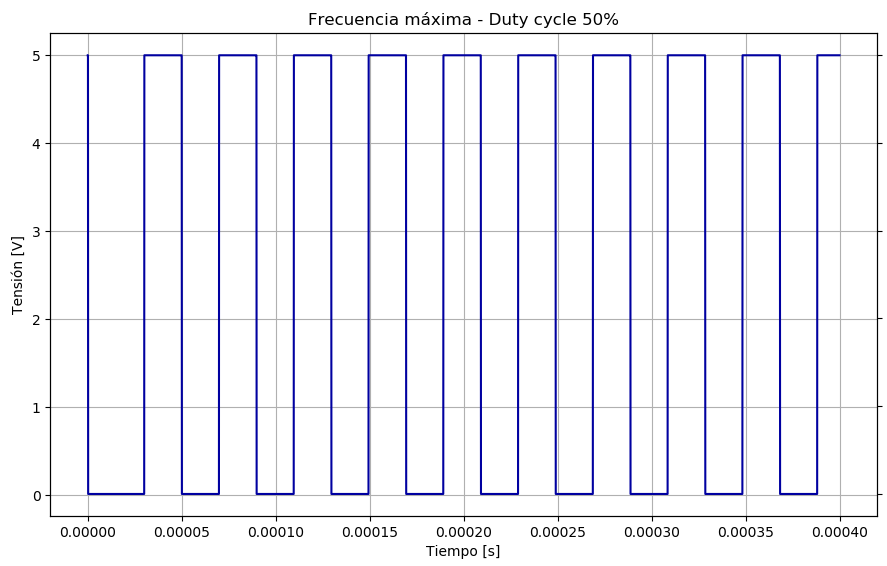
\includegraphics[width=\linewidth]{/ImagenesEjercicio1/DT50FMAX.png}
\caption{Onda simétrica con máxima frecuencia.}
\end{subfigure}
\begin{subfigure}[b]{.49\linewidth}
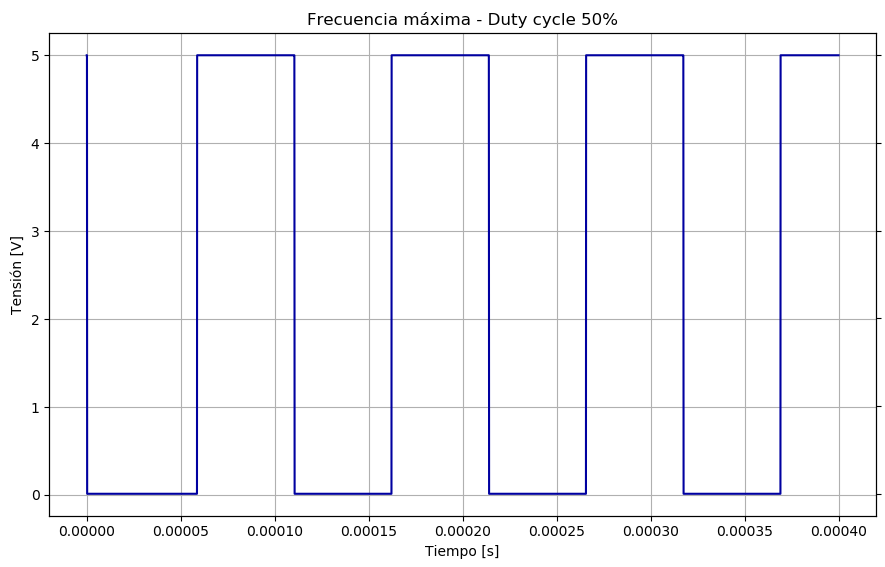
\includegraphics[width=\linewidth]{/ImagenesEjercicio1/DT50FMIN.png}
\caption{Onda simétrica con mínima frecuencia.}
\end{subfigure}

\begin{subfigure}[b]{.49\linewidth}
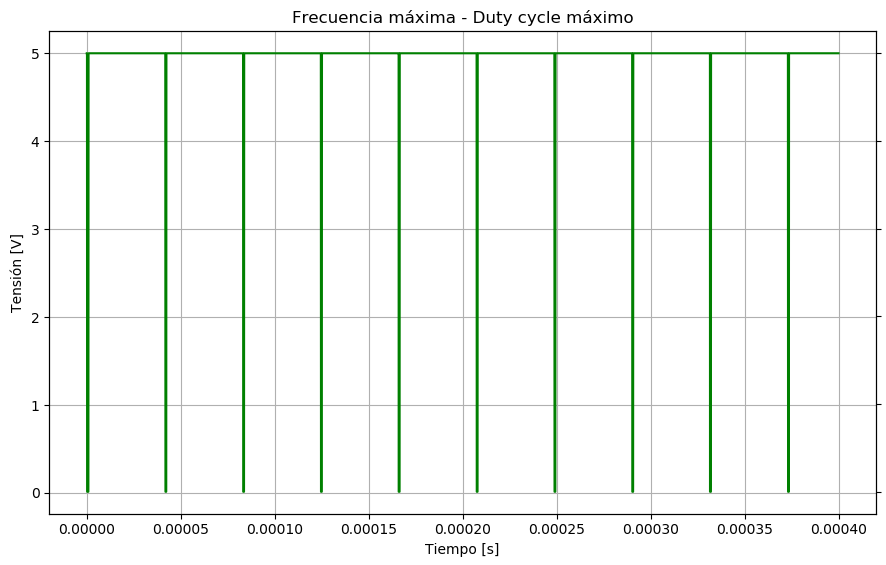
\includegraphics[width=\linewidth]{/ImagenesEjercicio1/DTMAXFMAX.png}
\caption{Máximo duty cycle con máxima frecuencia.}
\end{subfigure}
\begin{subfigure}[b]{.49\linewidth}
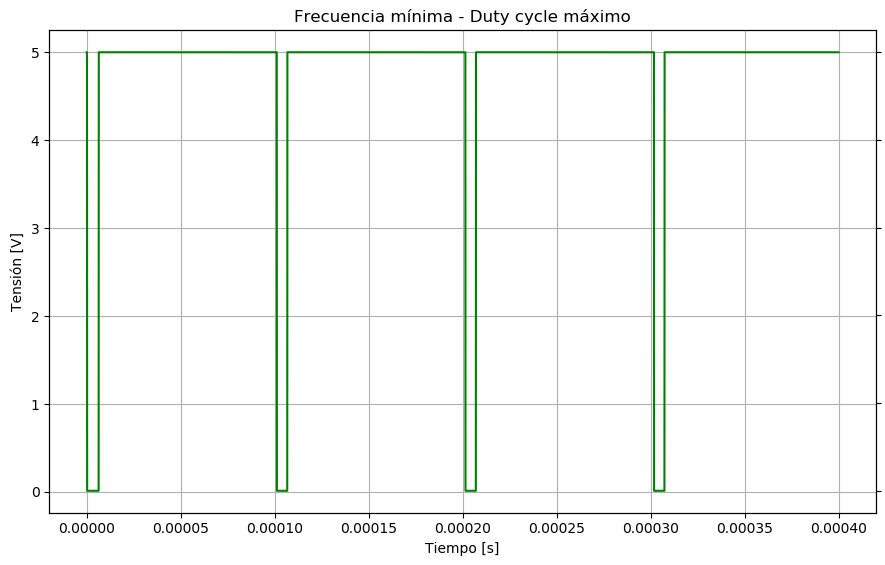
\includegraphics[width=\linewidth]{/ImagenesEjercicio1/DTMAXFMIN.png}
\caption{Máximo duty cycle con mínima frecuencia.}
\end{subfigure}

\begin{subfigure}[b]{.49\linewidth}
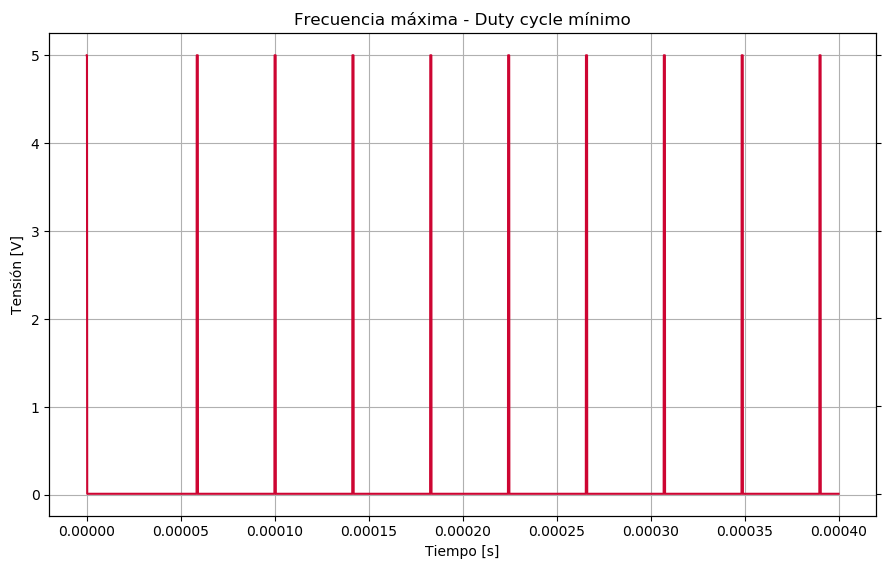
\includegraphics[width=\linewidth]{/ImagenesEjercicio1/DTMINFMAX.png}
\caption{Mínimo duty cycle con máxima frecuencia.}
\end{subfigure}
\begin{subfigure}[b]{.49\linewidth}
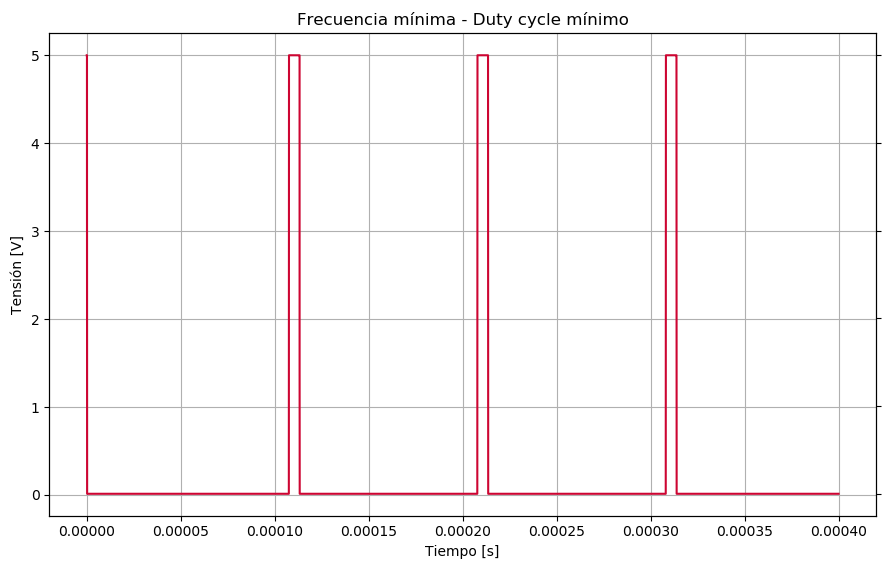
\includegraphics[width=\linewidth]{/ImagenesEjercicio1/DTMINFMIN.png}
\caption{Mínimo duty cycle con máxima frecuencia.}
\end{subfigure}

Finalmente, si se quisiera aumentar o decrementar la frecuencia de este oscilador en rangos mayores o menores a los detallados en un principio, basta simplemente con colocar un banco de capacitores con llaves de bypass para cada uno, de esta manera logrando un rango de variación de frecuencia muy grande, dado que la frecuencia depende proporcionalmente a la inversa de la capacitancia. Alternativamente, se pueden colocar jumpers para deshabilitar o habilitar cada capacitor. 

\end{figure}
